%
% Use the standard article template.
%
\documentclass{article}

% The geometry package allows for easy page formatting.
\usepackage{geometry}
\geometry{letterpaper}

% Load up special logo commands.
\usepackage{doc}

% Package for formatting URLs.
\usepackage{url}

% Packages and definitions for graphics files.
\usepackage{graphicx}
\usepackage{epstopdf}
\DeclareGraphicsRule{.tif}{png}{.png}{`convert #1 `dirname #1`/`basename #1 .tif`.png}

%
% Set the title, author, and date.
%
\title{Accelerometer data classification using Neural Networks}
\author{ Sameer, Shantanu, Rekah, Eera}
\date{}

%
% The document proper.
%
\begin{document}

% Add the title section.
\maketitle

% Add an abstract.
\abstract{
Human activity is a great source for building new kind of services that take the current status of the user into consideration.
Equipping a service provided by a phone application with the context of the user results in richer and more engaging services. In 
this work we present a neural based classifier that is able to detect the status of the human body from readings of 
accelerometers placed on different parts of the body. We show how different configuration of the neural network and 
data preprocessing can change the accuracy of our prediction, we also show how we can predict the movement using one 
accelerometer reading to simulate the effect of having a mobile device in users pocket or a smart watch attached to 
the user's wrist. To the best of our knowledge this is the first study that considers a single source of data and 
achieves (676876\%) accuracy. 
}

% Add various lists on new pages.
\pagebreak
\tableofcontents

\pagebreak
\listoffigures

\pagebreak
\listoftables

% Start the paper on a new page.
\pagebreak

%
% Body text.
%
\section{Introduction}
\label{introduction}

With the increasing use of smart mobile devices new opportunities are present for richer and more engaging services 
that cater to every need of its users. Most of these smart devices are equipped with accelerometers that give an
indication of of the relative position of the device and its user at any point in time. Using this data to identify the 
status of body movement provides an accurate record of the physical activity of the user which has applications related 
to the health care and interactive design for mobile devices' applications. 

In this work we seek to build a neural network based classifier that is able to correctly identify a pattern of human body 
movement from a series of readings, we discuss different design choices and report their impact on prediction accuracy. The 
rest of this report goes as follows; section~\ref{DataSet} describes the dataset we are using, section~\ref{accelerometer} 
provides a simple description of the inner workings of accelerometers for the inexperienced reader, section~\ref{meth} describes 
the methodology we used, section~\ref{conclusion} discusses a summary of the results we are getting and includes ideas for future work.

\section{Accelerometer}
\label{accelerometer} 
\DeclareGraphicsExtensions{.pdf,.png,.jpeg}

MAGIC MAGIC MAGIC OH MY GOD !!

\section{Data Set}
\label{DataSet}

Raw data we are using are based on the work by~\cite{ugulino2012wearable}. The data set report 8 hours of activity of 4 subject tests 
of varying age , weight, height and gender. Each subject provided two hours of activity of postures varying between (Standing,
sitting down, sitting , standing up and walking). The data provided is a continuous stream of reading from sensors placed of four 
parts of the body, waist, arm, leg and foot. Figure~\ref{acc_placement} shows the places of these accelerators~\cite{ugulino2012wearable}. 


\begin{figure}[h]
\centering
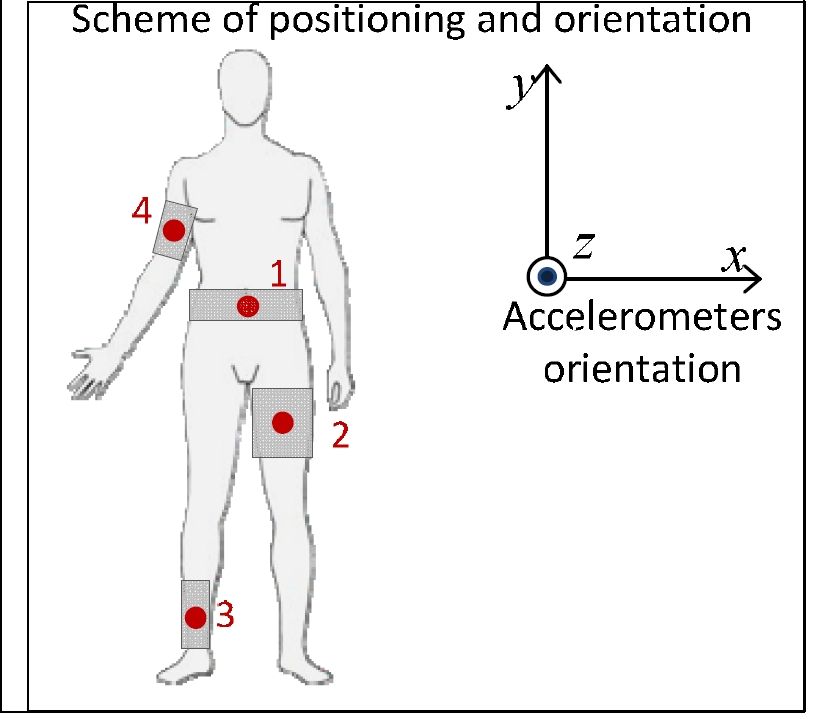
\includegraphics[width=2.5in]{acc_placement}
\caption{Accelerometer Placement}
\label{acc_placement}
\end{figure}
 

\section{Methodology}
\DeclareGraphicsExtensions{.pdf,.png,.jpeg}
\label{meth}

Previous work in detecting the body posture~\cite{ugulino2012wearable} used decision tree algorithms , namely C4.5,  with intensive 
data preprocessing and feature extraction before actually using the data for classification; work include finding the roll and 
pitch angles for the body and also the variance in roll and pitch . In this work we opted for doing as possible of data preprocessing
and to let the neural network the feature extraction. We try to train our network with the following variants:

\begin{enumerate}
  \item Using unprocessed rows and feeding them to the network, section~\ref{simple_rows} discusses that.
  \item Using deltas of two consecutive  rows or more than two rows, section~\ref{consecutive_rows} discusses that. 
  \item A person specific learner where we only do the training for one person for increased accuracy. 
  \item Use only one accelerometer to detect body posture. This gives a more realistic use case where the user only 
        has one source of data; a smart phone. Section~\ref{single_acc} discusses that.
  \item Using recurrent neural network to classify raw data. Section~\ref{rec_neural} discusses this work.
  \item Hello 
\end{enumerate}  

\subsection{Classification using raw rows}
\label{simple_rows}

\subsection{Consecutive Rows}
\label{consecutive_rows}
MAGIC MAGIC MAGIC.

\subsection{Single source of data} 
\label{single_acc}

\subsection{Recurrent neural network}
\label{rec_neural}

In this section we try to use recurrent Neural networks instead of feed forward 
networks to build a learner for the continuous data. Wu use Continuous time recurrent 
Neural networks.  

%\begin{figure}[h]
%\centering
%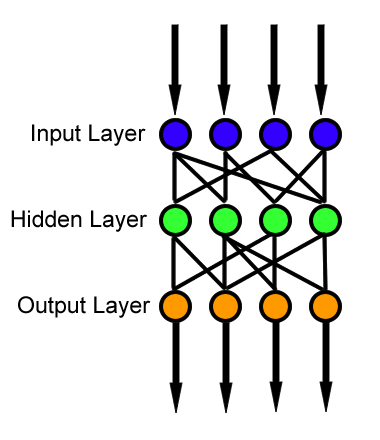
\includegraphics[width=2.5in]{feed_forward_neural_net}
%\captio{Feed forward network}
%\label{feed_forward}
%\end{figure}

\section {Conclusion}
\label{conclusion}

\section{Future Step for this work}
MAGIC MAGIC 

\begin{enumerate}
  \item Sameer
  \item is  
  \item the 
  \item Best
\end{enumerate}

% Generate the bibliography.
\bibliography{report}{}
\bibliographystyle{plain}
\end{document}
